\documentclass[tikz,border=3pt]{standalone}
\usepackage[utf8]{inputenc}
\usepackage[T1]{fontenc}
\usepackage{lmodern}
\renewcommand{\familydefault}{\sfdefault}
\usepackage{amsmath}
\usepackage{sansmath}\sansmath
\usepackage{pgfplots}\pgfplotsset{compat=1.18,/pgf/number format/use comma,/pgf/number format/1000 sep={.}}
\usetikzlibrary{arrows.meta,calc,positioning,decorations.pathmorphing,patterns}
% paleta del sitio
\definecolor{nar}{HTML}{E8680C}\definecolor{narc}{HTML}{FFB35C}\definecolor{hielo}{HTML}{FFF3E8}
\definecolor{tinta}{HTML}{1D1D1F}\definecolor{gris}{HTML}{6E6E73}\definecolor{lila}{HTML}{7C5CF0}
\definecolor{azul}{HTML}{2F6FD6}\definecolor{menta}{HTML}{17A673}\definecolor{coral}{HTML}{E8342A}
\pgfplotsset{base/.style={axis lines=left,grid=major,grid style={gris!20},tick label style={font=\small},label style={font=\small},axis line style={tinta!80}}}
\begin{document}
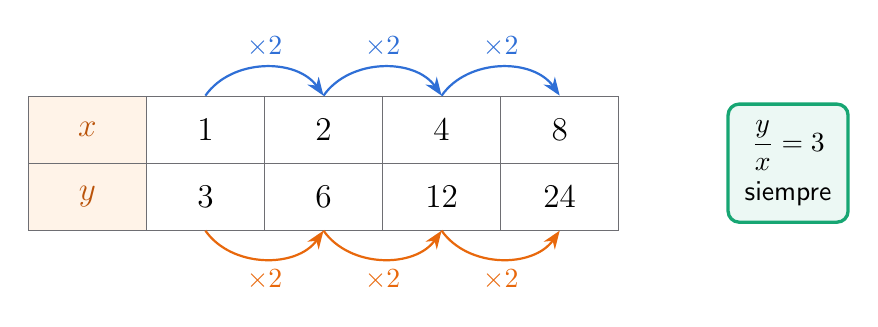
\begin{tikzpicture}[font=\large,
 c/.style={draw=gris,minimum width=1.5cm,minimum height=0.85cm},
 h/.style={c,fill=hielo,text=nar!80!black,font=\large\bfseries}]
\node[h] at (0,0) {$x$}; \node[h] at (0,-0.85) {$y$};
\foreach \v [count=\i] in {1,2,4,8} \node[c] (a\i) at (1.5*\i,0) {$\v$};
\foreach \v [count=\i] in {3,6,12,24} \node[c] (b\i) at (1.5*\i,-0.85) {$\v$};
\foreach \i/\j in {1/2,2/3,3/4} {
 \draw[-{Stealth},thick,azul] (a\i.north) to[bend left=55] node[above,font=\normalsize]{$\times 2$} (a\j.north);
 \draw[-{Stealth},thick,nar] (b\i.south) to[bend right=55] node[below,font=\normalsize]{$\times 2$} (b\j.south);}
\node[draw=menta,very thick,rounded corners,fill=menta!8,align=center,font=\normalsize,inner sep=6pt] at (8.9,-0.425) {$\dfrac{y}{x} = 3$\\[3pt] siempre};
\end{tikzpicture}
\end{document}
